\documentclass{article}
\usepackage{indentfirst}
\usepackage{float} 
\usepackage{graphicx}
\usepackage{amsmath}

\title{AJUSTE DE PREDICTOR PARA IMAGE SEGMENTATION DATA SET}
\author{Antonio José Blánquez Pérez, Diego Navarro Cabrera}
\date{Proyecto final Aprendizaje Automático - Universidad de Granada}

\begin{document}
 \setlength{\parskip}{1em} 

	\maketitle
	
	% Recordar plantearse cambiar los titulos de las versiones antes de entregar

	\section{Definición del problema y enfoque elegido}

	La base de datos seleccionada es Image Segmentation Data Set, creada por el Vision Group perteneciente a la Universidad de Massachusetts. Está formada por varias fotografías recogidas de 7 bases de datos que contienen distintos elementos al aire libre, los cuales son brickface(losa), sky(cielo), foliage(follaje), cement(cemento), window(ventana), path(camino) y grass(césped). Cada imagen ha sido segmentada a mano de manera que cada instancia de nuestra base de datos es una región de 3x3 píxeles de alguna de ellas, teniendo cada una 19 atributos relacionados con características como el color o el contraste. 
	\par
	Con esta información se pretende generar un modelo mediante técnicas de aprendizaje supervisado que prediga correctamente, dada una sección de 3x3 píxeles de una imagen, a que clase de las 7 antes mencionadas pertenece.
	
	\section{Argumentos a favor de la elección de los modelos}
	
	Se han elegido tres modelos candidatos para el problema que nos ocupa, uno lineal y dos no lineales. El modelo lineal ha sido seleccionado mediante validación cruzada entre dos posibilidades: Regresión Logística y Perceptrón, siendo la primera técnica la que mejor resultado proporciona y por tanto la seleccionada para comparar con los dos modelos no lineales. El modelo Perceptrón es un gran clasificador, sobre todo cuando los datos son linealmente separables, ya que si esto ocurre nos asegura una clasificación perfecta de los datos de la muestra de entrenamiento; siendo además, ayudado por el algoritmo Pocket, capaz de dar buenos resultados aún sin ser los datos linealmente separables. Regresion Logística sin embargo asigna las etiquetas a cada elemento a partir de la probabilidad que tiene de pertenecer a una clase o a otra, lo cual parece ser mejor que Perceptrón probablemente porque el conjunto de entrenamiento no sea ni se acerque a ser linealmente separable.
		
	Uno de los modelos no lineales que hemos escogido ha sido Boosting. La idea tras esta técnica es utilizar una gran cantidad de clasificadores simples, de manera que cada clasificador se centra en los errores del clasificador anterior. Uno de los atractivos de Boosting es su simpleza, tanto en dificultad como en complejidad, consiguiendo buenos resultados a pesar de ella. Inicialmente la varianza es muy baja, y con los pasos adecuados se puede conseguir bajar el sesgo en gran medida, por ello y por todas las ventajas de esta técnica esperamos conseguir buenos resultados.
	
	La otra elección de modelo no lineal ha sido Random Forest. Esta técnica se basa en boostrap para generar muestras y crear árboles de decision a partir de ellas. No obstante, para evitar que en todos los árboles se escojan inicialmente las mismas variables, selecciona para cada árbol un subconjunto de ellas aleatoriamente. Así, entre el bagging y esta característica conseguimos rebajar la varianza más que en el resto de técnicas basadas en árboles, que junto al bajo sesgo que consiguen los árboles de decisión, tenemos una técnica que puede proporcionar muy resultados, muy fiables, y además una gran eficiencia debido a su construcción.
	
	\section{Codificación de los datos de entrada para hacerlos útiles a los algoritmos}
	
	En principio los datos no necesitan ningún tipo de codificación para ser útiles en proceso de aprendizaje, no obstante se ha planteado la conversión de los datos a combinaciones cuadráticas de estos. Sin embargo, tras pruebas usando esta técnica, se ha visto que los resultados mejoran muy poco respecto los valores originales y por lo tanto se ha decidido usar estos últimos, ya que introducir tanta complejidad en el ajuste para una mejora tan irrelevante es incluso contraproducente.
	\par
	Si que ha sido necesario codificar la variables de clase, ya que originalmente están especificadas con el nombre del elemento. Para ello hemos creado una función $encodeLabels$ la cual recibe como parámetros el conjunto y un vector con las categorías; este último, si se omite, quedará como un vector vacío. El algoritmo que se usa es simple, para cada variable de clase, si encontramos una categoría nueva la añadimos al vector y cambia su valor el índice del nuevo elemento del vector, si ya lo está, tan solo cambia el valor por el índice de la categoría correspondiente; así se usa para generar el vector de categorías en el conjunto de entrenamiento y, con esa codificación, hacer la misma transformación en el conjunto de test. Al realizarse esta tarea en tiempo de ejecución no es necesario modificar estos valores en los archivos originales. La codificación obtenida, que será útil en posteriores análisis, es la siguiente: $0:BRICKFACE,\ 1:SKY,\ 2:FOLIAGE,\ 3:CEMENT,\ 4:WINDOW,\ 5:PATH,\ 6:GRASS$.
	\par
	Esta base de datos en concreto tiene una peculiaridad, y es que tiene una proporción entre el conjunto de entrenamiento y el de test remarcablemente anormales, ya que training consta de 210 instancias mientras que test tiene 10 veces más, 2100 instancias. Lo más probable es que esta proporción sea así porque se estima que esas 210 muestras (30 de cada clase) son suficientes para tener una imagen general de la fotografía que se quiere clasificar y por lo tanto son suficientes para ajustar el modelo. El gran número de instancias en el conjunto de prueba sirve para obtener una estimación fiable del error fuera de la muestra, ya que un 20\% o 30\% del tamaño del conjunto de entrenamiento podría ser poco incluso para un problema relativamente sencillo como este.
	
	\section{Valoración del interés de las variables}
	
	En cuanto a las variables medidas en cada instancia, todas parecen aportar información que uno podría considerar valiosa para identificar una imagen, y puesto que no es un número demasiado elevado de atributos no tenemos razones para intentar reducir la dimensionalidad del problema desechando algunas de ellas o usando una técnica de reducción como PCA.
	\par 
	Si que hay una variable de la que nos vamos a deshacer, pero esto es debido a que funciona como una constante que toma el mismo valor en todas las instancias, esta variable es el número de píxeles por región, que es 9 en todos los casos. Al ser una variable que no cambia de una instancia a otra no nos aporta ninguna información que pueda ser útil para nuestro modelo, por lo que eliminarla no afecta a la solución, pero si al tiempo de ejecución, que se ve reducido al tener que tratar con menos datos.
	
	\section{Normalización de las variables} % Diego
	
	Puesto que el rango de los atributos varia de unos a otros es importante reescalar cada uno de forma independiente para poder compararlos mejor y no darle más o menos peso a cada atributo en función de su tamaño. Para esto usaremos una escala min-max que para cada atributo $x_i$ perteneciente a la muestra i calcula:
	\begin{equation}
	x_i' = \frac{x_i-min}{max-min}
	\end{equation}
	\indent Donde min y max son los valores mínimo y máximo del atributo en toda la muestra.
	\par 
	Este tipo de escala mantiene la distribución de los valores, pero los ajusta a un rango entre 0 y 1.  Si supiéramos que los datos se siguen un tipo de distribución como la distribución normal podríamos usar otras formas de normalización, pero este no parece ser el caso, por lo que usar estas otras técnicas modificaría la distribución de la muestra y provocaría un peor ajuste.
	\par 
	Para evitar mezclar la información del conjunto de entrenamiento con la del de prueba aplicaremos este ajuste en cada conjunto de forma independiente, ya que si no no podríamos confiar en el valor de $E_{test}$ para estimar $E_{out}$.
	
	\section{Justificación de la función de pérdida usada}
	
	Como métrica de errores vamos a usar dos:
	\begin{enumerate}
		\item $zero\_one\_loss$, la cual es una medida estándar de error en clasificación. Ésta proporciona una medición de los valores que pertenecen a una clase concreta y el clasificador las ha etiquetado en otra, es decir, de los elementos mal clasificados. La hemos elegido porque es una medida simple y que proporciona claramente un valor real del error.
		\item Matrices de confusión, las cuales nos proporcionan información con la que podemos estudiar qué clases son las más problemáticas para nuestros modelos y sacar información más detallada a cerca de la precisión del ajuste.
	\end{enumerate}
	
	\section{Selección de técnicas y valoración de la idoneidad de cada una frente a otras alternativas}
	
	\subsection{Modelo Lineal}
	Para ajustar el modelo lineal vamos a usar la función de la biblioteca sklearn del gradiente descendente estocástico $SGDClassifier$. Vamos a comparar entre 2 modelos diferentes, y decidiremos cual es mejor en tiempo de ejecución. Los modelos que vamos a comparar son regresión logística y la implementación que usa la biblioteca del Perceptrón.
	\par 
	Usamos SGD como técnica	de ajuste porque es un algoritmo de optimización ámpliamente usado para ajustar todo tipo de modelos, y su implementación en scikit-learn nos facilitará su uso y el ajuste de todos sus posibles parámetros. 
	\subsection{Boosting}
	Como técnica de boosting vamos a usar gradient boosting mediante la función $GradientBoostingClassifier$, que aunque no use funciones stamp como se recomienda en el guión, funciona mucho mejor que $AdaBoost$ u otras funciones que si las usen. Esto se debe a que puesto que nuestro conjunto de datos de entrenamiento es muy pequeño y simple, necesitamos técnicas con una muy buena capacidad de aprendizaje y podemos permitirnos métodos más computacionalmente exigentes. 
	\subsection{Random Forest}
	En el caso de Random Forest vamos a usar la versión estándar de scikit-learn para clasificación: $RandomForestClassifier$, del módulo $ensemble$. Se plantean otras alternativas nombradas como árboles extremadamente aleatorizados, sin embargo en este caso no nos interesan ya que este conjunto de datos es lo suficientemente simple como para poder generar un número de árboles que nos garantice una buena varianza en un tiempo razonable. Es por esto por lo que no nos interesa una técnica que fuerza más la aleatoriedad en pos de bajar varianza a costa de sesgo.
	
	\section{Aplicación de la técnica: estimación de los parámetros, hiperparámetros y el error de generalización}
	
	Para ajustar los hiperparámetros de todos los modelos usaremos la función $GridSearchCV$ de la biblioteca scikit-learn, que recibe un conjunto de valores posibles para los distintos parámetros que se quieren ajustar y usa validación cruzada para determinar cual es la mejor combinación de dichos valores.
	\subsection{Modelo Lineal}
	Para el ajuste de los modelos lineales nos centraremos en 2 parámetros que ajustaremos con $GridSearchCV$: loss, que indicará el modelo ajustado, que podrá ser log (regresión logística) o perceptron, como ya se ha comentado antes; y el factor de regularización, que provocará una regularización más o menos agresiva en función de lo alto que sea.
	\par 
	A parte de estos parámetros, es importante determinar el tipo de regularización usada de la que hablaremos más adelante.
	\par 
	El resto de parámetros que usa la función sirven para acelerar el proceso de aprendizaje (a veces a costa de obtener peores resultados), fijar una solución inicial o determinar las condiciones de parada. Puesto que estos factores sirven más para reducir el tiempo de ejecución que para mejorar el ajuste, y dado que el tiempo de ejecución no es excesivamente alto, no hay necesidad de cambiar los valores que vienen asignados por defecto.
	\par 
	Al ejecutar el programa, la mejor combinación de parámetros nos da  $E_{val} = 0.1333$ y $E_{test} = 0.1238$, valores que no distan mucho del error dentro de la muestra $E_{in} = 0.0857$. Como era de esperar, $E_{val}$ es ligeramente mayor que $E_{test}$, ya que usa menos instancias de entrenamiento, aunque también hay que tener en cuenta un ligero margen por el ruido y la aleatoriedad de la técnica usada. Al tratarse de un problema con 7 clases podemos considerar un error cercano al 12\% como un buen comienzo, ya que la relativa simpleza de los modelos lineales va limitar la calidad de los resultados que obtengamos en muchos problemas.
	  \par 
	Como ya sabemos $E_{out}$ solo diferirá del valor de $E_{test}$ calculado en un infinitesimal de orden $\frac{1}{\sqrt{K}}$, siendo K el tamaño de test, que en nuestro caso es bastante grande, y que por lo tanto la diferencia entre $E_{out}$ y $E_{test}$ será muy pequeña y la podremos despreciar. Este razonamiento es valido tanto para este modelo como para los que veremos a continuación.
	
	\subsection{Boosting}
	El principal parámetro que determinará la calidad de nuestro modelo es el número de estimadores, que indicará el número de etapas de la fase de aprendizaje. Puesto que este método es bastante resistente al sobreajuste, no hará falta hacer muchas pruebas para ajustar este valor, puesto que podemos elegir un número que consideremos lo suficientemente alto sin miedo a pasarnos y obtener un mal ajuste. En este caso, el número elegido es 100, ya que a partir de este número no parece haber una diferencia significativa más allá de las variaciones posibles por la aleatoriedad del sistema.
	\par 
	Para regularizar usaremos 3 atributos principalmente, la tasa de aprendizaje, el tamaño de la submuestra que usamos para el entrenamiento de los estimadores, y el número máximo de atributos que se valoran en cada partición. Estimaremos su valor usando grid search, y en el siguiente apartado hablaremos con más detalle sobre el significado y la utilidad de estos atributos.
	\par 
	El resto de parámetros, al igual que con $SGDClassifier$, podemos decir que modificarlos no afectaría significativamente a la calidad del resultado, por lo que podemos dejarlos con sus valores por defecto.
	\par 
	En cuanto a los resultados que obtenemos al ejecutar el programa, tenemos  $E_{val} = 0.0571$, $E_{test} = 0.0571$ y $E_{in} = 0$. Al tratarse de un conjunto de entrenamiento muy pequeño y no muy complejo es normal que un modelo más potente como es gradient boosting sea capaz de reducir el error dentro de la muestra a 0, sin embargo,debido a las medidas de regularización tomadas y a que el error de prueba no está muy alejado del error de entrenamiento, podemos estar tranquilos de que no estamos sobreajustando más de lo debido nuestro modelo.
	
	\subsection{Random Forest}
	Uno de los principales parámetros a tener en cuenta en Random Forest es el número de árboles que se usarán, que en nuestro caso hemos comprobado que el más optimo es 100 debido a que el resultado deja de mejorar a partir de ese punto, entrenando aún así en un tiempo razonable. Otro parámetro a tener en cuenta es el criterio usado al elegir los atributos, teniendo las opciones del criterio Gini y el de la entropía.
	\par
	El segundo es el que hemos estudiado junto al algoritmo ID3, mientras que el primero tiene en cuenta la probabilidad de que un elemento elegido aleatoriamente quede mal etiquetado si lo hacemos también de manera aleatoria. Como a simple vista no queda claro qué técnica es mejor en este caso, se han sometido a validación cruzada, quedando seleccionado el criterio de la entropía.
	\par
	También existen una serie parámetros relacionados con el criterio de parada para establecer un conjunto de hoja. Esto nos interesa por dos motivos, principalmente para regularizar aunque también pueden ser útiles si tenemos problemas con el tiempo de ejecución, en este caso se ha establecido el máximo de profundidad en 8(se comentará más a fondo en el apartado posterior) y el resto no han sido necesarios. Por ello hemos creído conveniente dejar estos valores de manera que no limiten el proceder del algoritmo, coincidiendo con los valores por defecto.
	\par
	Adicionalmente es posible establecer cuantos atributos participan al ramificar el árbol. Tampoco es fácil de determinar cuántos darán el mejor resultado, por lo que se han sometido a validación cruzada las posibilidades de la raíz cuadrada del total, el logaritmo en base 2 y los porcentajes de 60, 70, 80 y 90\%, que son los que hemos creído más razonables. El resultado, lejos de sorprender, es que la raíz cuadrada da el mejor resultado, por algo es el valor por defecto y el que se usa usualmente para esta técnica. El resto de parámetros que proporciona la función usada no son interesantes para este estudio, por lo que se dejan por defecto.
	\par
	Tras la ejecución se han obtenido los siguiente resultados: $E_{val} = 0.0571$, $E_{test} = 0.0528$ y $E_{in} = 0.0047$. Podemos llegar a la misma conclusión que en el caso de Boosting, el error en la muestra tan bajo podría denotar un sobreajuste, sin embargo el modelo de entrenamiento es lo suficientemente simple para ajustar el error tan cercano a 0 con un modelo como Random Forest; $E_{test}$ es lo suficientemente bajo como para concluir que el resultado es satisfactorio, tan solo un error del 5.2\%.
	
	\section{Regularización}
	
	\subsection{Modelos Lineales}
	Puesto que estamos ante un problema en el que algunos atributos pueden ser más importantes que otros y no están del todo correlados entre si, la regularización Lasso es la mejor elección que podemos tomar. Este tipo de regularización limita el valor que puede tener la suma de los valores absolutos del peso de cada atributo, haciendo que algunos de ellos tiendan a 0 y por lo tanto se tengan menos en cuenta en el modelo. Esto permitirá que nuestra función se centre mejor en los elementos que mejor sirven para diferenciar las imágenes, reduciendo el ruido que aportarían otros atributos más innecesarios.
	\subsection{Boosting}
	Las principales formas de regularizar el proceso de ajuste de la función $GradientBoostingClassifier$ son 3 atributos. Por un lado, la tasa de aprendizaje indica cuanto aporta cada iteración al proceso de ajuste, y disminuyendo esta aportación podemos hacer que el ajuste se realice de forma más gradual y frenar o evitar el sobreajuste. 
	\par 
	Por otro lado, la función ofrece un parámetro que indica la fracción de instancias que se van a usar en el entrenamiento de los estimadores individuales, de forma que si se indica un número menor a 1.0 la función usa una versión estocástica del ajuste reduciendo la varianza del modelo.
	\par 
	Por último, el número máximo de atributos determina cuantos atributos se van a evaluar a la hora de buscar la mejor partición, y limitarlo obliga a escoger particiones subóptimas y, de forma similar al funcionamiento del gradiente descendente estocástico, dificulta caer en óptimos locales y reduce la varianza del modelo a cambio de un ligero aumento del sesgo.
	\subsection{Random Forest}
	En el caso de Random Forest es posible regularizar el proceso de ajuste estableciendo una profundidad máxima para los árboles o podándolos, optándose en este caso por la primera opción ya que es más simple y ha dado mejor resultado. Estas limitaciones sirven para regularizar debido a que un árbol empieza a tener sobreajuste cuando crece demasiado, esto es porque donde debería de haber un nodo hoja puede crearse otra estructura de ramas provocada por factores como el ruido. Con esto conseguimos evitar el sobreajuste a coste de algo de sesgo.
	\par
	En nuestro caso particular se ha decidido usar el parámetro $max_depth$ para limitar la profundidad máxima de los árboles de Random Forest por las razones ya comentadas, tras varias pruebas se ha elegido el valor 8, por lo que aunque no había demasiadas expectativas de sobreajuste lo aseguramos de esta manera.
	
	\section{Valoración de los resultados} % Hacer juntos al final
	Los resultados finales obtenidos para cada modelo son los siguientes:
	\begin{figure}[H]
	  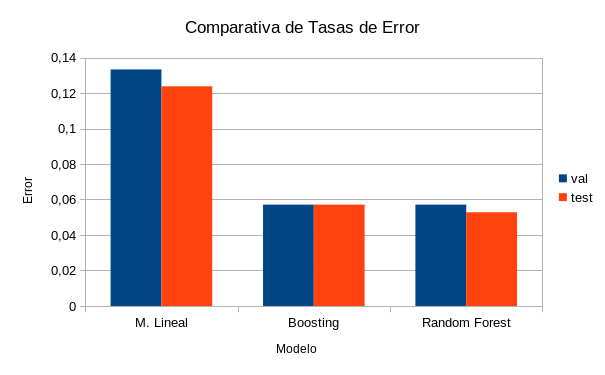
\includegraphics[width=\linewidth]{Imagenes/CE.png}
	  %\caption{Comparativa}
	  \label{fig:boat1}
	\end{figure}
	Como se puede ver, los modelos no lineales nos ofrecen un ajuste claramente mejor que el del modelo lineal, como era de esperar gracias a su mayor capacidad de separar los datos y a su propio diseño pensado para reducir la varianza y evitar el sobreajuste usando numerosos estimadores o arboles para producir una predicción fiable. 
	\par 
	Por otro lado, podríamos decir que el modelo que mejor resultado nos ha dado es Random Forest, sin embargo, la diferencia de este con Boosting es lo suficientemente pequeña como para que no podamos estar seguros de que esta sea una diferencia real y no solo un producto del azar inherente a estos modelos. Como se puede ver, tanto un modelo como el otro comparten el mismo $E_{val}$, a pesar de que el error de prueba de RF sea menor. Aun con todo, si tuviésemos que elegir un modelo de entre los que hemos usado, eligiríamos RF ya que aún con todo es el que mejor resultado nos ha dado.
	\par
	Estudiemos ahora las matrices de confusión(izquierda $E_{in}$, derecha ${E_{test}}$):
	
	\begin{equation}
		\begin{pmatrix}
			29 & 0 & 0 & 0 & 1 & 0 & 0\\
			0 & 30 & 0 & 0 & 0 & 0 & 0\\
			0 & 0 & 24 & 0 & 6 & 0 & 0\\
			0 & 0 & 1 & 23 & 2 & 4 & 0\\
			0 & 0 & 4 & 0 & 26 & 0 & 0\\
			0 & 0 & 0 & 0 & 0 & 30 & 0\\
			0 & 0 & 0 & 0 & 0 & 0 & 30
		\end{pmatrix}
		\begin{pmatrix}
		282 & 0 & 1 & 13 & 4 & 0 & 0\\
		0 & 300 & 0 & 0 & 0 & 0 & 0\\
		0 & 0 & 223 & 2 & 75 & 0 & 0\\
		1 & 1 & 3 & 202 & 26 & 67 & 0\\
		1 & 0 & 52 & 7 & 236 & 4 & 0\\
		0 & 0 & 0 & 0 & 0 & 300 & 0\\
		0 & 0 & 0 & 0 & 0 & 3 & 297
		\end{pmatrix}
	\end{equation}
	
	\begin{equation}
	\begin{pmatrix}
	30 & 0 & 0 & 0 & 0 & 0 & 0\\
	0 & 30 & 0 & 0 & 0 & 0 & 0\\
	0 & 0 & 30 & 0 & 0 & 0 & 0\\
	0 & 0 & 0 & 30 & 0 & 0 & 0\\
	0 & 0 & 0 & 0 & 30 & 0 & 0\\
	0 & 0 & 0 & 0 & 0 & 30 & 0\\
	0 & 0 & 0 & 0 & 0 & 0 & 30
	\end{pmatrix}
	\begin{pmatrix}
	281 & 0 & 0 & 16 & 3 & 0 & 0\\
	0 & 300 & 0 & 0 & 0 & 0 & 0\\
	1 & 0 & 270 & 4 & 25 & 0 & 0\\
	2 & 0 & 3 & 283 & 11 & 1 & 0\\
	1 & 0 & 29 & 22 & 248 & 0 & 0\\
	0 & 0 & 1 & 5 & 0 & 294 & 0\\
	1 & 0 & 1 & 0 & 0 & 1 & 297
	\end{pmatrix}
	\end{equation}
	
	\begin{equation}
	\begin{pmatrix}
	29 & 0 & 0 & 0 & 1 & 0 & 0\\
	0 & 30 & 0 & 0 & 0 & 0 & 0\\
	0 & 0 & 30 & 0 & 0 & 0 & 0\\
	0 & 0 & 0 & 30 & 0 & 0 & 0\\
	0 & 0 & 0 & 0 & 30 & 0 & 0\\
	0 & 0 & 0 & 0 & 0 & 30 & 0\\
	0 & 0 & 0 & 0 & 0 & 0 & 30
	\end{pmatrix}
	\begin{pmatrix}
	286 & 0 & 0 & 11 & 3 & 0 & 0\\
	0 & 300 & 0 & 0 & 0 & 0 & 0\\
	2 & 1 & 276 & 8 & 13 & 0 & 0\\
	2 & 0 & 0 & 278 & 17 & 3 & 0\\
	2 & 0 & 31 & 9 & 258 & 0 & 0\\
	0 & 0 & 0 & 6 & 0 & 294 & 0\\
	0 & 0 & 0 & 0 & 0 & 3 & 297
	\end{pmatrix}
	\end{equation}
	
	En primer lugar analizaremos las matrices en el caso del modelo lineal $(2)$, donde podemos ver que los errores se concentran claramente, tanto en entrenamiento como en test, en las clases FOLIAGE, CEMENT y WINDOW, dando el resto muy buenos resultados aun con modelos lineales. En el caso de CEMENT hablamos incluso de un tercio de los elementos mal clasificados, por lo que será en estas tres clases donde deberá destacar el uso de modelos no lineales. El resto de elementos mal clasificados no es demasiado remarcable, son errores asumibles en un resultado satisfactorio. Es posible concluir también a partir de estos detalles que las imágenes de las clases FOLIAGE y WINDOW parecen las más difíciles de separar, la clase CEMENT sin embargo parece confundirse también con WINDOW y con PATH.
	\par 
	Si comparamos el comportamiento anterior con el presente en Boosting y RF $(3)(4)$ se pueden ver distintas mejoras. La más evidente es que el problema con la clase CEMENT, aunque sigue quedando algo presente, ha mejorado en gran medida; si antes no era para nada un buen resultado ahora podemos afirmar que es etiquetado de manera satisfactoria dentro de un margen de error asumible. De la misma manera se puede observar y confirmar que la dificultad de separar las clases FOLIAGE y WINDOW queda presente, añadiendo el aliciente de que con estos dos modelos la clasificación en la muestra de entrenamiento es prácticamente perfecta. Esto deja patente que es difícil separar ambas clases bajo los atributos manejados en este estudio y que por tanto, junto a la clase CEMENT y en algún caso BRICKFACE, son las que afectan principalmente al error ya estudiado. No obtstante los resultados, tanto de Boosting como de RF, mejoran en gran medida al modelo lineal y proporcionan un ajuste, al menos en nuestra opinión, de calidad.
	
	\section{Conclusiones}
	Como ya se ha hablado antes, cada modelo se ha ajustado buscando los mejores parámetros posibles y se han tomado las medidas necesarias para asegurar que el error calculado con el conjunto de prueba es lo más fiable posible, de forma que el modelo que nos devuelva una menor tasa de error debería ser el mejor de entre las soluciones posibles. Dicho esto, la naturaleza aleatoria del proceso siempre puede afectar ligeramente a los resultados , y puesto que solo podemos estimar $E_{out}$, nunca saber su valor real, bajo condiciones ligeramente diferentes podríamos estimar como óptimos otros parámetros e incluso otros modelos, ya que como hemos dicho antes, la diferencia entre Boosting y Random Forest no es tan grande como para asegurar que uno sea mejor que otro.
	\par 
	Otra razón para creer que la solución obtenida es lo mejor posible es que tanto Boosting como RF tienen un error dentro de la muestra prácticamente igual a 0 (RF solo clasifica mal 1 muestra) en ausencia(al menos aparente) de sobreajuste, por lo que la única forma de ajustar mejor el error fuera de esta sería reducir aún más la diferencia entre $E_{in}$ y $E_{out}$, algo en lo que estos modelos ya son especialmente buenos, por lo que cuesta creer la obtenida como una mala solución, sobre todo teniendo en cuenta la limitada extensión del conjunto de entrenamiento.
	
	
\end{document}